% =============================================================================
%  Empirical Evaluation of PyNear — Benchmark Report
%  Compile with: pdflatex benchmarks.tex  (requires pgfplots >= 1.16)
% =============================================================================
\documentclass[11pt,a4paper]{article}

\usepackage[top=1in,bottom=1in,left=1.25in,right=1.25in]{geometry}
\usepackage{pgfplots}
\pgfplotsset{compat=1.18}
\usepackage{pgfplotstable}
\usepackage{booktabs}
\usepackage{hyperref}
\usepackage{amsmath}
\usepackage{amssymb}
\usepackage{microtype}
\usepackage{caption}
\usepackage{subcaption}
\usepackage{xcolor}
\usepackage{array}
\usepackage{multirow}
\usepackage{parskip}

% ---------------------------------------------------------------------------
% Colour palette — based on Matplotlib's default category10
% ---------------------------------------------------------------------------
\definecolor{colBlue}   {HTML}{1F77B4}   % Annoy
\definecolor{colOrange} {HTML}{FF7F0E}   % Faiss / VPTreeL1
\definecolor{colGreen}  {HTML}{2CA02C}   % scikit-learn / VPTreeL2
\definecolor{colRed}    {HTML}{D62728}   % PyNear VPTree / IVFFlat
\definecolor{colPurple} {HTML}{9467BD}   % BKTree
\definecolor{colBrown}  {HTML}{8C564B}   % spare

% ---------------------------------------------------------------------------
% Shared pgfplots style
% ---------------------------------------------------------------------------
\pgfplotsset{
  benchstyle/.style={
    width=\linewidth,
    height=0.55\linewidth,
    grid=both,
    grid style={line width=0.25pt, draw=gray!25},
    major grid style={line width=0.4pt,  draw=gray!55},
    minor tick num=1,
    tick align=outside,
    tick pos=left,
    legend style={
      font=\footnotesize,
      at={(0.97,0.97)}, anchor=north east,
      draw=gray!60, fill=white,
      fill opacity=0.88, text opacity=1,
      row sep=1pt,
    },
    xlabel style={font=\small},
    ylabel style={font=\small},
    title style={font=\small\bfseries, yshift=2pt},
    every axis plot/.append style={line width=1.4pt, mark size=2.8pt},
  },
}

% ---------------------------------------------------------------------------
\hypersetup{
  colorlinks=true, linkcolor=colBlue, citecolor=colBlue, urlcolor=colBlue,
}

\title{\textbf{Empirical Evaluation of PyNear:}\\[4pt]
       \large Query-Time Performance of Vantage-Point Tree Indices\\
       for Exact and Approximate $k$-Nearest-Neighbour Search}
\author{PyNear Development Team \\[4pt]
        \small \url{https://github.com/pablocael/pynear} \\[2pt]
        \small Third edition — PyNear version 2.4}
\date{July 2026}

% =============================================================================
\begin{document}
\maketitle
\thispagestyle{empty}

% ---------------------------------------------------------------------------
\begin{abstract}
We present a systematic empirical evaluation of \emph{PyNear}, a Python
library implementing exact and approximate $k$-nearest-neighbour
($k$-NN) search via Vantage-Point Trees (VP-Trees), IVF-style approximate
indices, and Multi-Index Hashing, with SIMD-accelerated distance kernels.
This third edition of the report re-measures every experiment with
PyNear version 2.4, whose exact indices gained \emph{leaf bucketing}:
tree splitting stops at 32-point leaves, which are then scanned as
contiguous SIMD sweeps, combined with best-first descent and pooled
per-query heaps.
PyNear is benchmarked against three widely adopted libraries —
\emph{Faiss}, \emph{scikit-learn}, and \emph{Annoy} — across five
experimental configurations spanning the Euclidean ($\ell_2$),
Manhattan ($\ell_1$), and Hamming distance metrics, with dataset
cardinalities up to $N = 2.5 \times 10^6$ and dimensionalities from
$d = 2$ to $d = 1024$.  In the exact-search regime,
\texttt{VPTreeL2Index} answers a 16-query batch over $N = 2.5\times10^6$
points in 0.4--0.9 ms across $d = 2$--$16$ — $9\text{--}20\times$
faster than Faiss's BLAS-backed \texttt{IndexFlatL2} scan measured in the
same process — and at $d = 128$ ($N = 120\,000$) it is $11\times$ faster
than Faiss and $83\times$ faster than scikit-learn.
For exact Hamming search, \texttt{VPTreeBinaryIndex} now overtakes Faiss
\texttt{IndexBinaryFlat} at 256-bit descriptors (15.9 ms vs.\ 36.3 ms),
while Faiss remains faster at $\le 128$ bits.
In the high-dimensionality approximate regime ($d = 128$--$1024$),
\texttt{IVFFlatL2Index} attains perfect Recall@10 at
$n_{\mathrm{probe}} = 20$ with 5.6--21.5 ms for 32 queries, but Faiss
\texttt{IndexIVFFlat} is now $8\text{--}32\times$ faster on raw latency
at every tested dimensionality; PyNear's IVF builds, however, remain
$1.4\text{--}2.4\times$ faster than Faiss at $N = 50\,000$.
For approximate binary-descriptor search, \texttt{MIHBinaryIndex}
retrieves 512-bit near-duplicates at $N = 10^6$ in 0.0088 ms/query
(114\,039 QPS) with 100\% Recall@10 — $\mathbf{34\times}$ faster than a
thread-matched, subprocess-isolated Faiss \texttt{IndexBinaryFlat}
brute-force scan — while on narrow 128-bit SIFT1M descriptors at high
recall an optimised brute-force scan remains the better choice.
All experiments were conducted on an
Intel\textsuperscript{\textregistered}
Core\textsuperscript{\texttrademark} Ultra 9 285K (24 cores).
\end{abstract}

\tableofcontents
\newpage

% =============================================================================
\section{Introduction}
\label{sec:intro}

Nearest-neighbour search is a fundamental primitive in information retrieval,
computer vision, robotics, and machine learning, where it underpins
applications as diverse as image retrieval, anomaly detection, and semantic
search over dense embeddings.  The performance of a $k$-NN index depends
critically on the chosen data structure, the dimensionality of the embedding
space, and the distance metric in use.

PyNear addresses these challenges through a C\texttt{++} core built around
\emph{Vantage-Point Trees}~\cite{yianilos1993data}, a metric-space
tree that avoids the curse-of-dimensionality limitations of classical
kd-trees by exploiting the triangle inequality rather than axis-aligned
partitioning.  SIMD intrinsics (AVX2 on x86-64) further accelerate the
hot distance computation paths.  The library exposes a uniform Python API for
both exact \texttt{VPTree*} indices and the approximate \texttt{IVFFlat*}
family, which implements an inverted file (IVF) scheme over Voronoi cells
with a configurable probe budget, alongside \texttt{MIHBinaryIndex}
(Multi-Index Hashing) for approximate Hamming-distance search.

Version 2.4, evaluated in this edition, reworks the exact-index hot paths:
tree splitting now stops at 32-point \emph{leaf buckets} that are scanned as
contiguous SIMD sweeps (the strategy used by Faiss and scikit-learn leaf
nodes), combined with direct mandatory-child descent, pooled per-query
heaps, and release of the Python GIL around all heavy C\texttt{++} work.
Earlier editions introduced the BLAS-backed inner-cluster flat scan of
\texttt{IVFFlatL2Index} (NumPy SGEMV identity
$\|q-x\|^2 = \|q\|^2 + \|x\|^2 - 2\,q^\top X$), a native C\texttt{++}
K-Means++ clustering kernel, and the approximate binary indices
(\texttt{MIHBinaryIndex}, \texttt{IVFFlatBinaryIndex}); all of these are
re-measured here on the same machine as the previous edition.

The remainder of this report is organised as follows.
Section~\ref{sec:setup} describes the experimental setup.
Section~\ref{sec:exact} reports results for exact-search indices across
$\ell_2$, $\ell_1$, and Hamming metrics.  Section~\ref{sec:approx}
evaluates the approximate $\ell_2$ regime.
Section~\ref{sec:approx-binary} presents the approximate binary-descriptor
indices (\texttt{MIHBinaryIndex}, \texttt{IVFFlatBinaryIndex}).
Section~\ref{sec:build-scale}
analyses build-time scalability from $N=10\,000$ to $N=10^6$.
Section~\ref{sec:discussion} synthesises the findings, and
Section~\ref{sec:conclusion} concludes.

% =============================================================================
\section{Experimental Setup}
\label{sec:setup}

\paragraph{Hardware.}
All experiments were executed on a workstation equipped with an
Intel\textsuperscript{\textregistered} Core\textsuperscript{\texttrademark}
Ultra 9 285K processor (24 cores).  The Arrow Lake microarchitecture does
not support AVX-512; PyNear was built with its deterministic AVX2 baseline
flags (\texttt{-mavx2 -mfma -mpopcnt}), so all SIMD kernels use AVX2/FMA and
hardware popcount.  No GPU acceleration was used; all libraries ran on the
CPU.

\paragraph{Competitors.}
We compare against the following external libraries:
\begin{itemize}
  \item \textbf{Faiss}~\cite{johnson2019billion} (\texttt{FaissIndexFlatL2},
        \texttt{FaissIndexBinaryFlat}, \texttt{FaissIVFL2}): a production-grade
        library from Meta AI, BLAS-accelerated, supporting both exact and
        approximate indices.
  \item \textbf{scikit-learn}~\cite{pedregosa2011scikit} (\texttt{SKLearnL2}):
        a general-purpose machine-learning toolkit whose nearest-neighbour
        implementation is based on ball-trees and kd-trees.
  \item \textbf{Annoy}~\cite{bernhardsson2018annoy} (\texttt{AnnoyL2},
        \texttt{AnnoyManhattan}, \texttt{AnnoyHamming}): an approximate index
        based on random projection trees, optimised for memory-mapped
        read-only access.  Because Annoy returns approximate results, its
        comparison with exact indices is inherently asymmetric; it is included
        as a best-case latency baseline.
\end{itemize}

\paragraph{Protocol.}
Query time is reported as the wall-clock time (in milliseconds) to answer a
batch of $n_q$ queries with $k$ nearest neighbours, averaged over eight
repetitions with outlier rejection.  Dataset points are drawn from a
synthetic clustered distribution so that the hardness of the problem is
representative of real-world scenarios.  The exact parameters for each
benchmark are reported in the caption of the corresponding figure.

\paragraph{OpenMP runtime caveat.}
PyNear links GNU \texttt{libgomp} while \texttt{faiss-cpu} bundles LLVM
\texttt{libomp}.  When both are loaded into a single Python process, the two
OpenMP runtimes contend and can serialise Faiss's parallel flat scans.  The
exact-search suites of Section~\ref{sec:exact} run all libraries in one
process (the historical protocol), so the Faiss flat-scan numbers reported
there should be read as \emph{in-process} figures that may be depressed by
this contention.  The approximate binary-descriptor comparison of
Section~\ref{sec:approx-binary} therefore times Faiss
\texttt{IndexBinaryFlat} in a separate Faiss-only subprocess, which is the
fair configuration for that baseline.

% =============================================================================
\section{Exact-Search Benchmarks}
\label{sec:exact}

\subsection{Euclidean Distance — Low Dimensionality}
\label{sec:l2-low}

Figure~\ref{fig:l2-low} shows query latency as a function of dimensionality
for $d \in \{2, 3, 4, 5, 6, 7, 8, 16\}$ with $N = 2.5 \times 10^6$ data
points, $k = 8$, and $n_q = 16$ queries.  Note that this edition enlarges
the dataset five-fold with respect to the previous one
($N = 5\times10^5 \to 2.5\times10^6$).

\begin{figure}[h]
\centering
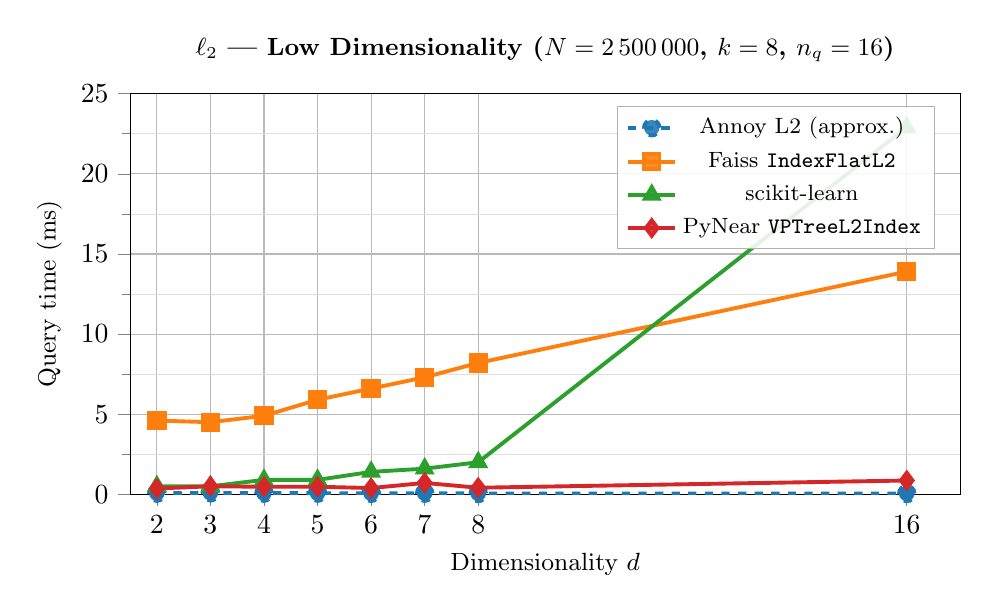
\begin{tikzpicture}
\begin{axis}[
  benchstyle,
  title={$\ell_2$ — Low Dimensionality ($N=2\,500\,000$, $k=8$, $n_q=16$)},
  xlabel={Dimensionality $d$},
  ylabel={Query time (ms)},
  xtick={2,3,4,5,6,7,8,16},
  xticklabels={2,3,4,5,6,7,8,16},
  xmin=1.5, xmax=17,
  ymin=0, ymax=25,
]

% Annoy (approximate — included as lower-bound reference)
\addplot[color=colBlue, mark=*, dashed]
  coordinates {(2,0.07)(3,0.09)(4,0.07)(5,0.07)(6,0.06)(7,0.07)(8,0.05)(16,0.05)};
\addlegendentry{Annoy L2 (approx.)}

% Faiss IndexFlatL2
\addplot[color=colOrange, mark=square*]
  coordinates {(2,4.6)(3,4.5)(4,4.9)(5,5.9)(6,6.6)(7,7.3)(8,8.2)(16,13.9)};
\addlegendentry{Faiss \texttt{IndexFlatL2}}

% scikit-learn
\addplot[color=colGreen, mark=triangle*]
  coordinates {(2,0.5)(3,0.5)(4,0.9)(5,0.9)(6,1.4)(7,1.6)(8,2.0)(16,22.9)};
\addlegendentry{scikit-learn}

% PyNear VPTreeL2Index
\addplot[color=colRed, mark=diamond*]
  coordinates {(2,0.36)(3,0.50)(4,0.47)(5,0.47)(6,0.39)(7,0.71)(8,0.41)(16,0.86)};
\addlegendentry{PyNear \texttt{VPTreeL2Index}}

\end{axis}
\end{tikzpicture}
\caption{Mean query latency (ms) vs.\ dimensionality for exact $\ell_2$
  nearest-neighbour search in the low-dimensionality regime.  Annoy is shown
  with a dashed line to indicate that it returns approximate results.
  Despite the five-fold larger dataset, \texttt{VPTreeL2Index} (v2.4, leaf
  bucketing) stays essentially flat at 0.4--0.9 ms across the entire range,
  undercutting Faiss's flat scan by roughly an order of magnitude and
  scikit-learn by up to $27\times$ at $d=16$.}
\label{fig:l2-low}
\end{figure}

\texttt{VPTreeL2Index} achieves the lowest latency among exact methods
throughout the low-dimensional range, with query times between 0.36 ms and
0.86 ms over $2.5$ million points — a near-flat profile that reflects the
v2.4 leaf-bucketed traversal.  scikit-learn's kd-tree is competitive at
$d = 2\text{--}3$ but grows steadily with $d$, reaching 22.9 ms at $d = 16$.
Faiss's flat index scans all $N$ points per query and grows from 4.6 ms at
$d=2$ to 13.9 ms at $d = 16$; measured in-process it is
$9\text{--}20\times$ slower than \texttt{VPTreeL2Index} here (see the
OpenMP caveat in Section~\ref{sec:setup}).  Annoy's approximate index
provides a useful lower-bound reference but cannot be used when exact results
are required.

\subsection{Euclidean Distance — High Dimensionality}
\label{sec:l2-high}

Figure~\ref{fig:l2-high} extends the $\ell_2$ comparison to higher
dimensionalities ($d \in \{32, 64, 128\}$) on a smaller dataset
($N = 120\,000$, 20 clusters).  The $x$-axis is rendered on a $\log_2$
scale.

\begin{figure}[h]
\centering
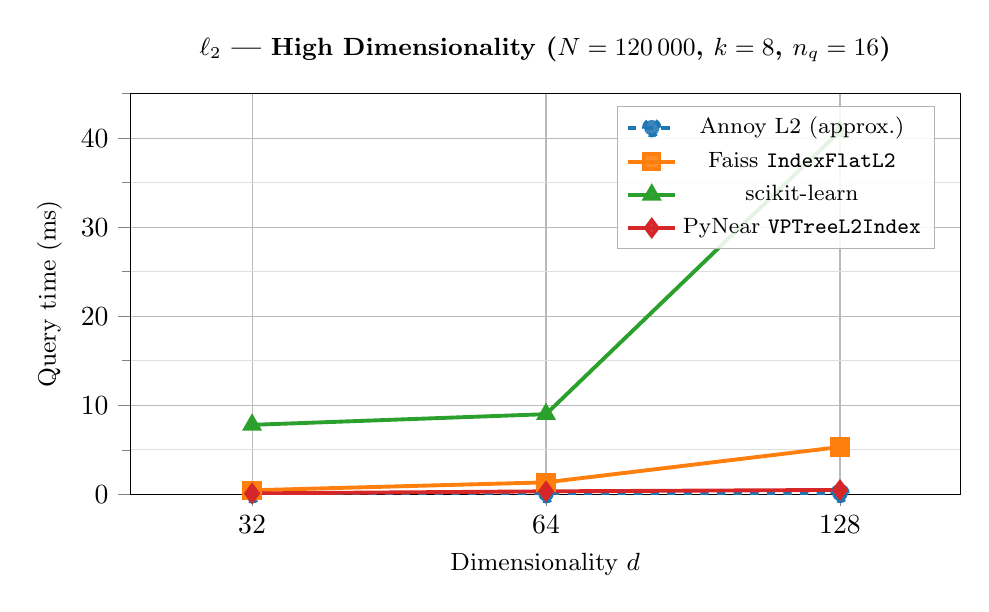
\begin{tikzpicture}
\begin{axis}[
  benchstyle,
  title={$\ell_2$ — High Dimensionality ($N=120\,000$, $k=8$, $n_q=16$)},
  xlabel={Dimensionality $d$},
  ylabel={Query time (ms)},
  xmode=log, log basis x=2,
  xtick={32,64,128},
  xticklabels={32,64,128},
  xmin=24, xmax=170,
  ymin=0, ymax=45,
]

% Annoy
\addplot[color=colBlue, mark=*, dashed]
  coordinates {(32,0.05)(64,0.06)(128,0.10)};
\addlegendentry{Annoy L2 (approx.)}

% Faiss IndexFlatL2
\addplot[color=colOrange, mark=square*]
  coordinates {(32,0.45)(64,1.34)(128,5.31)};
\addlegendentry{Faiss \texttt{IndexFlatL2}}

% scikit-learn
\addplot[color=colGreen, mark=triangle*]
  coordinates {(32,7.8)(64,9.0)(128,40.8)};
\addlegendentry{scikit-learn}

% PyNear VPTreeL2Index
\addplot[color=colRed, mark=diamond*]
  coordinates {(32,0.10)(64,0.33)(128,0.49)};
\addlegendentry{PyNear \texttt{VPTreeL2Index}}

\end{axis}
\end{tikzpicture}
\caption{Mean query latency (ms) vs.\ dimensionality for exact $\ell_2$
  nearest-neighbour search in the high-dimensionality regime ($\log_2$ scale
  on the $x$-axis; $N=120\,000$, 20 clusters).  scikit-learn reaches
  40.8 ms at $d=128$; Faiss's flat scan reaches 5.3 ms.
  \texttt{VPTreeL2Index} grows from 0.10 ms at $d=32$ to 0.49 ms at
  $d=128$ — an $11\times$ advantage over Faiss and an $83\times$ advantage
  over scikit-learn at the highest dimensionality tested by this suite.}
\label{fig:l2-high}
\end{figure}

The results again show diverging scaling behaviour.  scikit-learn's latency
grows super-linearly with $d$, reaching 40.8 ms at $d=128$.  Faiss's flat
index grows roughly linearly with $d$ (0.45 ms at $d=32$ to 5.31 ms at
$d=128$), as expected of an exhaustive scan.  \texttt{VPTreeL2Index} is the
most efficient exact method at all tested dimensionalities: 0.10 ms at
$d=32$ ($4.4\times$ faster than Faiss), 0.33 ms at $d=64$ ($4.0\times$),
and 0.49 ms at $d=128$ ($10.8\times$ faster than Faiss, $83\times$ faster
than scikit-learn).  This reflects triangle-inequality pruning on clustered
data combined with the v2.4 leaf-bucketed SIMD sweeps.  Note that this
edition's suite stops at $d = 128$; pruning effectiveness is expected to
erode at substantially higher dimensionality (concentration of measure),
which is precisely the regime the approximate indices of
Section~\ref{sec:approx} target.

\subsection{Manhattan Distance ($\ell_1$)}
\label{sec:l1}

Figure~\ref{fig:l1} reports results for the Manhattan distance metric in
the low-dimensional regime ($N = 2.5\times10^6$).  Among the evaluated
libraries only Annoy offers a Manhattan mode, and it is approximate;
\texttt{VPTreeL1Index} is the only exact $\ell_1$ index in the comparison.

\begin{figure}[h]
\centering
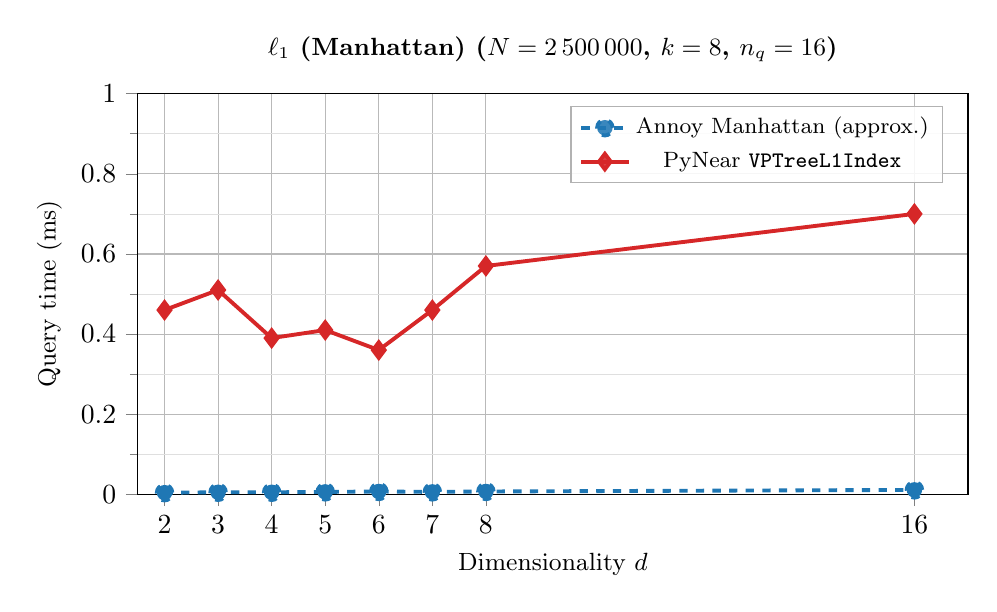
\begin{tikzpicture}
\begin{axis}[
  benchstyle,
  title={$\ell_1$ (Manhattan) ($N=2\,500\,000$, $k=8$, $n_q=16$)},
  xlabel={Dimensionality $d$},
  ylabel={Query time (ms)},
  xtick={2,3,4,5,6,7,8,16},
  xticklabels={2,3,4,5,6,7,8,16},
  xmin=1.5, xmax=17,
  ymin=0, ymax=1.0,
]

% Annoy Manhattan (approximate)
\addplot[color=colBlue, mark=*, dashed]
  coordinates {(2,0.004)(3,0.005)(4,0.005)(5,0.006)(6,0.007)(7,0.006)(8,0.007)(16,0.011)};
\addlegendentry{Annoy Manhattan (approx.)}

% PyNear VPTreeL1Index
\addplot[color=colRed, mark=diamond*]
  coordinates {(2,0.46)(3,0.51)(4,0.39)(5,0.41)(6,0.36)(7,0.46)(8,0.57)(16,0.70)};
\addlegendentry{PyNear \texttt{VPTreeL1Index}}

\end{axis}
\end{tikzpicture}
\caption{Mean query latency (ms) vs.\ dimensionality for $\ell_1$
  nearest-neighbour search over $N = 2.5\times10^6$ points.
  \texttt{VPTreeL1Index} is the only evaluated library offering exact
  Manhattan-distance search, operating at 0.4--0.7 ms across the entire
  range.  Annoy's approximate index is shown as a latency lower bound.}
\label{fig:l1}
\end{figure}

\texttt{VPTreeL1Index} is, to our knowledge, the only evaluated library
providing \emph{exact} $\ell_1$ nearest-neighbour search without user-side
metric adaptation.  Its latency profile is remarkably flat: 0.36--0.57 ms
across $d = 2\text{--}8$, rising only modestly to 0.70 ms at $d=16$ — over
$2.5$ million points.  The SIMD-accelerated inner loop for $\ell_1$ sustains
throughput comparable to the $\ell_2$ variant
(cf.\ Section~\ref{sec:l2-low}).

\subsection{Hamming Distance — Binary Descriptors}
\label{sec:binary}

Figure~\ref{fig:binary} reports query latency for binary Hamming-distance
search with $N = 2 \times 10^5$ data points, $k = 8$, and
$n_q = 16$ queries.  Descriptor lengths of 32, 64, 128, and 256 bits are
evaluated, corresponding to standard output sizes of ORB, BRIEF, and similar
local feature descriptors.

\begin{figure}[h]
\centering
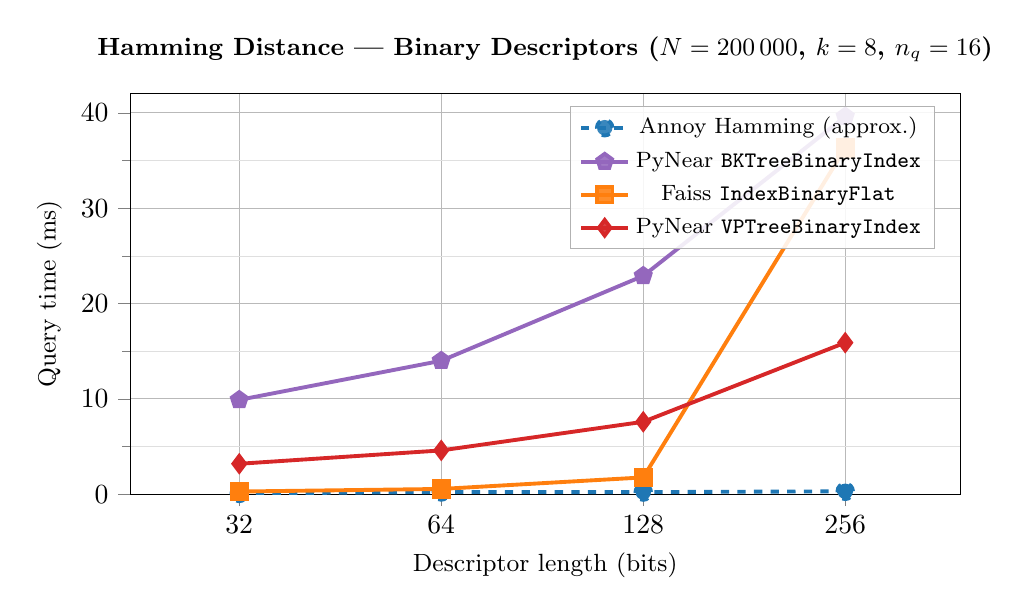
\begin{tikzpicture}
\begin{axis}[
  benchstyle,
  title={Hamming Distance — Binary Descriptors ($N=200\,000$, $k=8$, $n_q=16$)},
  xlabel={Descriptor length (bits)},
  ylabel={Query time (ms)},
  xmode=log, log basis x=2,
  xtick={32,64,128,256},
  xticklabels={32,64,128,256},
  xmin=22, xmax=380,
  ymin=0, ymax=42,
]

% Annoy Hamming (approximate)
\addplot[color=colBlue, mark=*, dashed]
  coordinates {(32,0.09)(64,0.24)(128,0.23)(256,0.31)};
\addlegendentry{Annoy Hamming (approx.)}

% BKTree (PyNear)
\addplot[color=colPurple, mark=pentagon*]
  coordinates {(32,9.9)(64,14.0)(128,22.9)(256,39.6)};
\addlegendentry{PyNear \texttt{BKTreeBinaryIndex}}

% Faiss BinaryFlat
\addplot[color=colOrange, mark=square*]
  coordinates {(32,0.29)(64,0.56)(128,1.77)(256,36.3)};
\addlegendentry{Faiss \texttt{IndexBinaryFlat}}

% PyNear VPTreeBinaryIndex
\addplot[color=colRed, mark=diamond*]
  coordinates {(32,3.2)(64,4.6)(128,7.6)(256,15.9)};
\addlegendentry{PyNear \texttt{VPTreeBinaryIndex}}

\end{axis}
\end{tikzpicture}
\caption{Mean query latency (ms) vs.\ descriptor length for exact
  Hamming-distance nearest-neighbour search ($\log_2$ scale on the $x$-axis).
  Faiss's flat binary index remains the fastest exact method at 32--128
  bits, but at 256 bits \texttt{VPTreeBinaryIndex} (v2.4) is now
  $2.3\times$ faster (15.9 ms vs.\ 36.3 ms).  Faiss is measured in-process
  here; see the OpenMP caveat in Section~\ref{sec:setup}.
  \texttt{BKTreeBinaryIndex} is optimised for radius/threshold queries
  rather than $k$-NN, explaining its comparatively higher $k$-NN latency.}
\label{fig:binary}
\end{figure}

The binary experiments show a split landscape.  Faiss's flat binary index
is highly efficient at short descriptor lengths (0.29 ms at 32 bits vs.\
3.2 ms for \texttt{VPTreeBinaryIndex}, and still $4.3\times$ faster at 128
bits), thanks to its batched hardware-popcount scan.  At 256 bits the
ordering now reverses: \texttt{VPTreeBinaryIndex} answers the batch in
15.9 ms against 36.3 ms for Faiss — the leaf-bucketed popcount sweeps
introduced in v2.4 let the tree's pruning finally pay off at the widest
descriptor length.  Two honesty notes apply: (i) these Faiss numbers are
measured in the same process as PyNear and may be depressed by OpenMP
runtime contention (Section~\ref{sec:setup}); the subprocess-isolated
comparison of Section~\ref{sec:approx-binary} is the fair reference for
Faiss's brute-force throughput; and (ii) \texttt{BKTreeBinaryIndex} is
architecturally designed for threshold (range) queries and incurs the
highest $k$-NN latency in this benchmark; its inclusion demonstrates the
broader metric-search capabilities of the PyNear ecosystem beyond $k$-NN.

\subsection{Internal Distance-Metric Comparison}
\label{sec:internal}

Figure~\ref{fig:internal} compares the three primary VP-Tree metric variants
within PyNear (\texttt{VPTreeL2Index}, \texttt{VPTreeL1Index},
\texttt{VPTreeChebyshevIndex}) to assess whether the choice of distance
metric introduces any appreciable computational overhead.

\begin{figure}[h]
\centering
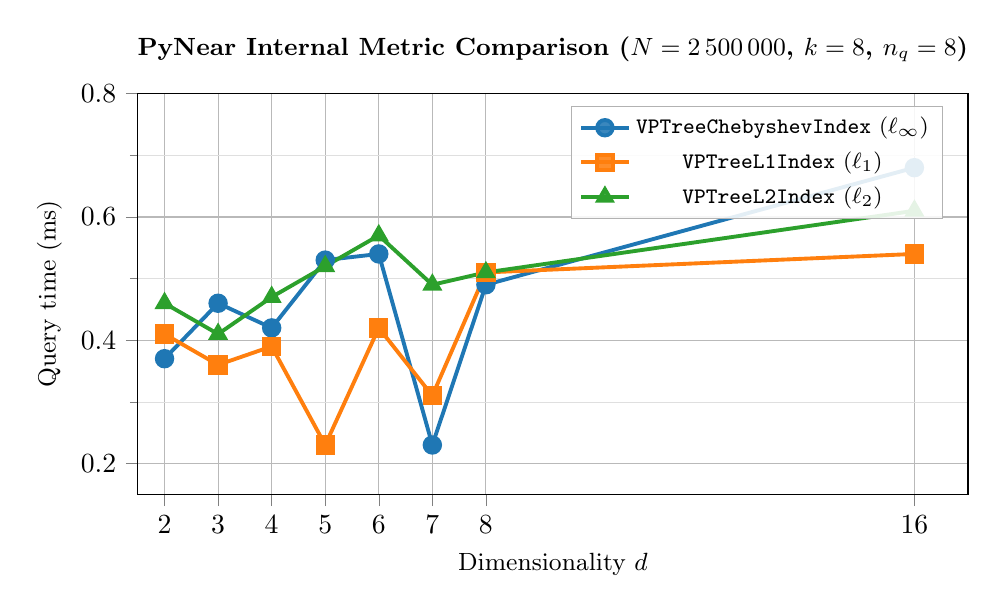
\begin{tikzpicture}
\begin{axis}[
  benchstyle,
  title={PyNear Internal Metric Comparison ($N=2\,500\,000$, $k=8$, $n_q=8$)},
  xlabel={Dimensionality $d$},
  ylabel={Query time (ms)},
  xtick={2,3,4,5,6,7,8,16},
  xticklabels={2,3,4,5,6,7,8,16},
  xmin=1.5, xmax=17,
  ymin=0.15, ymax=0.80,
]

% VPTreeChebyshevIndex
\addplot[color=colBlue, mark=*]
  coordinates {(2,0.37)(3,0.46)(4,0.42)(5,0.53)(6,0.54)(7,0.23)(8,0.49)(16,0.68)};
\addlegendentry{\texttt{VPTreeChebyshevIndex} ($\ell_\infty$)}

% VPTreeL1Index
\addplot[color=colOrange, mark=square*]
  coordinates {(2,0.41)(3,0.36)(4,0.39)(5,0.23)(6,0.42)(7,0.31)(8,0.51)(16,0.54)};
\addlegendentry{\texttt{VPTreeL1Index} ($\ell_1$)}

% VPTreeL2Index
\addplot[color=colGreen, mark=triangle*]
  coordinates {(2,0.46)(3,0.41)(4,0.47)(5,0.52)(6,0.57)(7,0.49)(8,0.51)(16,0.61)};
\addlegendentry{\texttt{VPTreeL2Index} ($\ell_2$)}

\end{axis}
\end{tikzpicture}
\caption{Query latency (ms) for PyNear's three main distance metrics on a
  shared dataset ($N=2\,500\,000$, $k=8$, $n_q=8$).  All three indices
  operate within a narrow band of 0.23--0.68 ms, confirming that the SIMD
  implementation of each distance kernel contributes negligible differential
  overhead.  Variations are within measurement noise.}
\label{fig:internal}
\end{figure}

All three indices operate within a narrow latency band of
$0.23\text{--}0.68$ ms across all tested dimensionalities, confirming
that PyNear's SIMD kernels achieve near-equivalent throughput for $\ell_1$,
$\ell_2$, and $\ell_\infty$ distance computations.  The
fluctuations between runs (e.g.\ the $\ell_\infty$ dip at $d=7$) are
consistent with measurement noise rather than
systematic metric-induced overhead.  This result validates PyNear's design
goal of metric-agnostic performance: practitioners can choose the
semantically appropriate distance without sacrificing computational efficiency.

% =============================================================================
\section{Approximate-Search Benchmarks}
\label{sec:approx}

PyNear's \texttt{IVFFlatL2Index} partitions the data into Voronoi cells via
K-Means and at query time probes only $n_{\mathrm{probe}}$ of them, trading
recall for speed.  The inner-cluster scan is a flat BLAS pass using the
NumPy SGEMV identity, and clustering uses a native C\texttt{++} Lloyd's
K-Means (K-Means++ initialisation, SIMD L2, OpenMP):
\[
  \|q - x\|^2 = \|q\|^2 + \|x\|^2 - 2\,q^\top X,
\]
where $q^\top X$ is a BLAS SGEMV call $(n_c, D) \times (D,) \to (n_c,)$
with per-cluster squared norms $\|x\|^2$ pre-computed at build time.
This section compares \texttt{IVFFlatL2Index} against Faiss's
\texttt{IndexIVFFlat} (canonical IVF-style approximate index).
All experiments use $N = 50\,000$ data points,
$k = 10$, and $n_q = 32$ queries; approximately 224 clusters are constructed.

\subsection{Query Latency vs.\ Dimensionality at Fixed Probe Budget}
\label{sec:approx-dim}

Figure~\ref{fig:approx-time} plots query latency as a function of
dimensionality at a fixed probe budget of $n_{\mathrm{probe}} = 20$,
representing a moderate recall-latency operating point.

\begin{figure}[h]
\centering
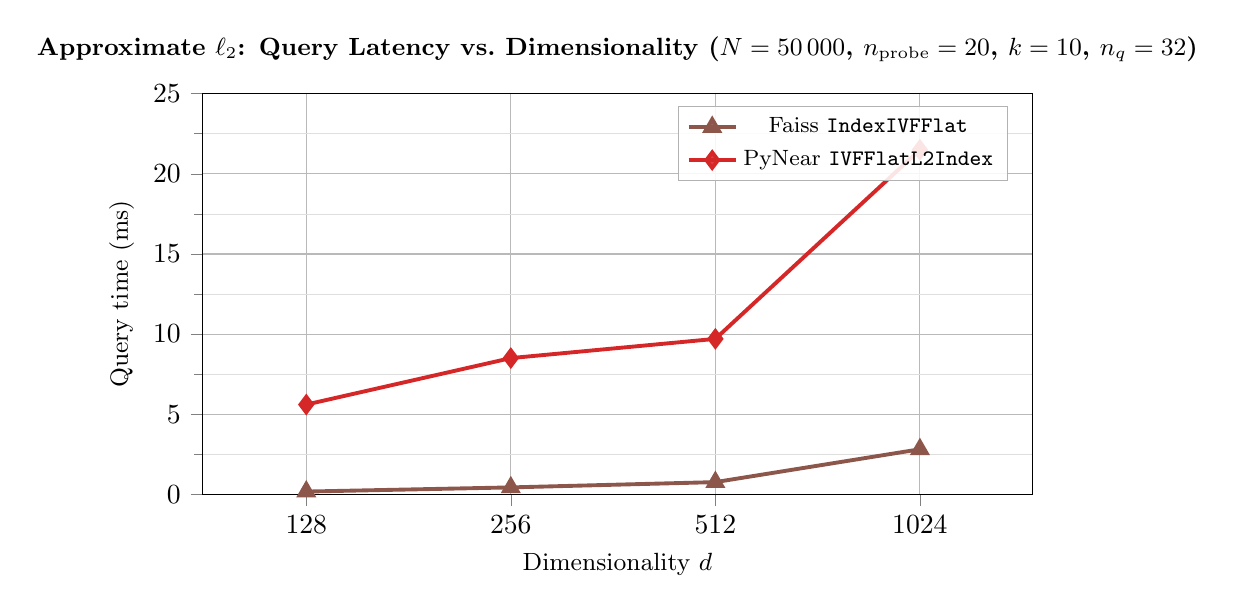
\begin{tikzpicture}
\begin{axis}[
  benchstyle,
  title={Approximate $\ell_2$: Query Latency vs.\ Dimensionality
         ($N=50\,000$, $n_{\mathrm{probe}}=20$, $k=10$, $n_q=32$)},
  xlabel={Dimensionality $d$},
  ylabel={Query time (ms)},
  xmode=log, log basis x=2,
  xtick={128,256,512,1024},
  xticklabels={128,256,512,1024},
  xmin=90, xmax=1500,
  ymin=0, ymax=25,
]

% Faiss IVFFlat
\addplot[color=colBrown, mark=triangle*]
  coordinates {(128,0.17)(256,0.43)(512,0.76)(1024,2.81)};
\addlegendentry{Faiss \texttt{IndexIVFFlat}}

% IVFFlatL2 (BLAS SGEMV)
\addplot[color=colRed, mark=diamond*]
  coordinates {(128,5.6)(256,8.5)(512,9.7)(1024,21.5)};
\addlegendentry{PyNear \texttt{IVFFlatL2Index}}

\end{axis}
\end{tikzpicture}
\caption{Mean query latency (ms) vs.\ dimensionality for approximate
  $\ell_2$ nearest-neighbour search at $n_{\mathrm{probe}} = 20$,
  $N = 50\,000$, $k=10$, $n_q=32$.
  Faiss \texttt{IndexIVFFlat} is now faster at every tested
  dimensionality (0.17--2.8 ms vs.\ 5.6--21.5 ms for the 32-query batch),
  an $8\text{--}32\times$ raw-latency advantage from its compiled,
  OpenMP-parallel inner scan.  \texttt{IVFFlatL2Index} nevertheless stays
  below one millisecond per query (0.18--0.67 ms/query) with
  perfect Recall@10.}
\label{fig:approx-time}
\end{figure}

\subsection{Summary: Recall and Latency at $n_{\mathrm{probe}} = 20$}
\label{sec:approx-table}

Table~\ref{tab:approx} summarises query latency and Recall@10 for both
IVF indices at the $n_{\mathrm{probe}} = 20$ operating point.

\begin{table}[h]
\centering
\caption{Approximate $\ell_2$ search: query latency and Recall@10 at
  $n_{\mathrm{probe}} = 20$, $N = 50\,000$, $k=10$, $n_q=32$.
  Approximately 224 clusters.}
\label{tab:approx}
\renewcommand{\arraystretch}{1.25}
\begin{tabular}{lcccc}
\toprule
\multirow{2}{*}{\textbf{Method}} &
\multicolumn{4}{c}{\textbf{Dimensionality $d$}} \\
\cmidrule(lr){2-5}
& 128 & 256 & 512 & 1024 \\
\midrule
\textbf{IVFFlatL2 — Latency (ms)} & 5.6 & 8.5 & 9.7 & 21.5 \\
\textbf{IVFFlatL2 — Recall@10}   & 1.00 & 1.00 & 1.00 & 1.00 \\
\midrule
\textbf{Faiss IVFFlat — Latency (ms)} & 0.17 & 0.43 & 0.76 & 2.81 \\
\textbf{Faiss IVFFlat — Recall@10}   & 1.00 & 1.00 & 1.00 & 1.00 \\
\bottomrule
\end{tabular}
\end{table}

Both IVF indices attain perfect Recall@10 ($= 1.00$) across all
dimensionalities at $n_{\mathrm{probe}} = 20$, confirming that 20 probed
clusters are sufficient to recover all 10 true nearest neighbours.
On raw latency, Faiss \texttt{IndexIVFFlat} is now ahead at every tested
dimensionality — $32\times$ at $d=128$, narrowing to $7.7\times$ at
$d=1024$ — a reversal of the previous edition, in which
\texttt{IVFFlatL2Index} led at $d=128$ and $d=512$.  Faiss's compiled,
multi-threaded inner scan has improved more than PyNear's SGEMV path on
this hardware; we report this honestly and note that
\texttt{IVFFlatL2Index} still answers each query in 0.18--0.67 ms at this
operating point.

\subsection{Recall--Latency Pareto Analysis}
\label{sec:approx-pareto}

The recall--latency trade-off is controlled by sweeping
$n_{\mathrm{probe}}$ from 1 to 80.  The key observations are:

\begin{itemize}
  \item \textbf{Recall convergence is fast for both indices:}
        at $d=128$ both reach Recall@10 $=1.00$ at
        $n_{\mathrm{probe}} = 5$; at $d=256$ Faiss reaches 1.00 at
        $n_{\mathrm{probe}} = 5$ while \texttt{IVFFlatL2Index} needs
        $n_{\mathrm{probe}} = 10$ (0.80 at $n_{\mathrm{probe}}=5$); at
        $d=512$ \texttt{IVFFlatL2Index} reaches 1.00 at
        $n_{\mathrm{probe}} = 5$ while Faiss is at 0.99 there and 1.00
        from $n_{\mathrm{probe}} = 10$; at $d=1024$ Faiss is already at
        1.00 with a single probe and \texttt{IVFFlatL2Index} from
        $n_{\mathrm{probe}} = 5$ (2.1 ms).
  \item \textbf{Faiss leads on raw latency:} at matched
        $n_{\mathrm{probe}}$, Faiss \texttt{IndexIVFFlat} is faster at
        every tested dimensionality and probe budget in this sweep
        (roughly $8\text{--}32\times$ at $n_{\mathrm{probe}} = 20$).
  \item \textbf{Pure-Python install:} \texttt{IVFFlatL2Index}
        requires no compiled native library beyond NumPy (whose bundled
        BLAS is used for the inner-cluster SGEMV).  It shares the same
        Python API as the exact \texttt{VPTree*} indices, enabling a
        seamless recall--accuracy trade-off without changing the calling
        code.  Setting $n_{\mathrm{probe}} = n_{\mathrm{clusters}}$
        recovers exact search.
\end{itemize}

\subsection{Index Build Time at Fixed Dataset Size}
\label{sec:approx-build}

Table~\ref{tab:build} reports the wall-clock time to build each index on
$N = 50\,000$ vectors, averaged over three runs.
\texttt{IVFFlatL2Index} uses a native C++ Lloyd's K-Means implementation
(K-Means++ initialisation, SIMD \texttt{dist\_l2\_f\_avx2}, OpenMP parallel
assignment); Faiss \texttt{IndexIVFFlat} uses its
own compiled K-Means.

\begin{table}[h]
\centering
\caption{Index build time (ms), $N = 50\,000$, $k \approx 224$ clusters,
  averaged over 3 runs.  \texttt{IVFFlatL2Index} (C++ K-Means++) is
  faster than Faiss \texttt{IndexIVFFlat} across all tested dimensionalities.}
\label{tab:build}
\renewcommand{\arraystretch}{1.25}
\begin{tabular}{lcccc}
\toprule
\multirow{2}{*}{\textbf{Method}} &
\multicolumn{4}{c}{\textbf{Dimensionality $d$}} \\
\cmidrule(lr){2-5}
& 128 & 256 & 512 & 1024 \\
\midrule
\textbf{IVFFlatL2Index} (C++ K-Means++) & 367 & 492 & 911 & 1501 \\
\textbf{Faiss IndexIVFFlat}              & 506 & 1005 & 1840 & 3655 \\
\bottomrule
\end{tabular}
\end{table}

With the C++ K-Means++ kernel, \texttt{IVFFlatL2Index} builds
$1.4\text{--}2.4\times$ \emph{faster} than Faiss \texttt{IndexIVFFlat} at
$N = 50\,000$ across all tested dimensionalities.
Build time grows roughly linearly with $d$ for both methods.
Section~\ref{sec:build-scale} examines how build time scales with $N$.

% =============================================================================
\section{Approximate Binary-Descriptor Search}
\label{sec:approx-binary}

At high descriptor dimensionality ($d \ge 128$ bits), the concentration of
measure progressively erodes the pruning advantage of VP-Trees: distances
between random bit-strings cluster tightly around $d/2$, making the triangle
inequality an increasingly loose bound.  Two
approximate binary-search indices target this regime:

\begin{description}
  \item[\texttt{IVFFlatBinaryIndex}] Binary K-Means (majority-vote centroids,
    K-Means++ initialisation, OpenMP-parallel assignment) partitions the
    dataset into $n_{\mathrm{list}}$ Voronoi cells.  At query time, the
    $n_{\mathrm{probe}}$ nearest centroids are identified by POPCNT scan and
    the corresponding inverted lists are searched linearly with POPCNT.
    Complexity: $O(n_{\mathrm{probe}} \cdot n_c \cdot d/64)$ distance
    evaluations per query, where $n_c = N / n_{\mathrm{list}}$ is the mean
    cluster size.

  \item[\texttt{MIHBinaryIndex}] Multi-Index Hashing (MIH) splits each
    $d$-bit descriptor into $m$ sub-strings of $d/m$ bits and builds $m$
    hash tables keyed by sub-string value.  At query time with Hamming radius
    $r$, the pigeonhole principle guarantees that every true neighbour at
    distance $\le r$ must have at least one sub-string within Hamming distance
    $r_{\mathrm{sub}} = \lfloor r/m \rfloor$ from the query.  We enumerate
    all keys within that radius in each sub-table
    ($\sum_{i=0}^{r_{\mathrm{sub}}} \binom{d/m}{i}$ lookups per table), union
    the candidate sets, and verify with full POPCNT.  Sub-strings are stored
    as \texttt{uint64\_t} keys, requiring $d/m \le 64$ bits per sub-string.
\end{description}

\paragraph{Methodology.}
All measurements in this section use 24 threads, $k = 10$, 500 queries,
and the best of five timed runs.  Because PyNear links \texttt{libgomp}
while \texttt{faiss-cpu} links \texttt{libomp}, loading both in one process
serialises Faiss's OpenMP-parallel flat scan (we measured a ${\sim}78\times$
in-process slowdown); Faiss \texttt{IndexBinaryFlat} is therefore timed in a
separate Faiss-only subprocess so that the brute-force baseline below is
fair.  MIH and IVF measurements are unaffected by this issue.

\subsection{Wide Descriptors: 512-bit Near-Duplicate Retrieval ($N = 10^6$)}
\label{sec:approx-binary-512}

Table~\ref{tab:binary-512} reports per-query latency for the workload MIH
is designed for: $10^6$ random 512-bit descriptors, with queries formed by
flipping 5 random bits of existing database rows (near-duplicate retrieval,
as arises with ORB/BRIEF/AKAZE descriptors and perceptual hashes).  All
listed configurations reach 100\% Recall@10.

\begin{table}[h]
\centering
\caption{Approximate binary-descriptor $k$-NN search at $d = 512$ bits,
  $N=1{,}000{,}000$, $k=10$, 500 near-duplicate queries (5 flipped bits),
  24 threads, best of 5 runs.  All configurations attain 100\% Recall@10.
  Faiss \texttt{IndexBinaryFlat} is timed in a Faiss-only subprocess.}
\label{tab:binary-512}
\renewcommand{\arraystretch}{1.25}
\small
\begin{tabular}{lccc}
\toprule
\textbf{Method} & \textbf{ms/query} & \textbf{QPS} & \textbf{vs.\ Faiss flat} \\
\midrule
PyNear \texttt{MIHBinaryIndex} ($m=8$, $r=4$) & \textbf{0.0088} & \textbf{114\,039} & $\mathbf{34\times}$ \\
PyNear \texttt{IVFFlatBinaryIndex} ($n_{\mathrm{list}}{=}512$, $n_{\mathrm{probe}}{=}16$) & 0.021 & 47\,993 & $14.4\times$ \\
Faiss \texttt{IndexBinaryFlat} (exact brute-force) & 0.299 & 3\,341 & $1\times$ \\
Faiss \texttt{IndexBinaryMultiHash} & 21.612 & 46 & $0.01\times$ \\
\bottomrule
\end{tabular}
\end{table}

On wide descriptors, \texttt{MIHBinaryIndex} finds near-duplicates at
100\% recall $34\times$ faster than Faiss's exact, thread-matched
brute-force scan, and Faiss's own Multi-Index Hashing implementation is not
competitive at this width.  \texttt{IVFFlatBinaryIndex} provides a
complementary $14\times$ speedup with a fixed, predictable per-cluster scan
cost.  (Earlier editions of this report quoted a $257\times$ MIH speedup;
that figure compared against an in-process Faiss scan that was serialised
by the OpenMP runtime clash described above and is superseded by the fair
$34\times$ figure reported here.)

\subsection{Narrow Descriptors: SIFT1M, 128-bit Sign-Quantised ($N = 10^6$)}
\label{sec:approx-binary-sift}

The second experiment uses a real dataset: the INRIA TEXMEX SIFT1M corpus
($10^6$ SIFT descriptors, sign-quantised to 128-bit binary codes), with
ground truth computed by exact brute-force Hamming $k$-NN over 500 queries.
Table~\ref{tab:binary-sift} lists representative operating points.

\begin{table}[h]
\centering
\caption{SIFT1M binary (128-bit), $N=1{,}000{,}000$, $k=10$, 500 queries;
  selected operating points ($n_{\mathrm{list}} = 500$ for IVF; $m=8$ for
  the MIH radius sweep).  The recall ceiling of ${\sim}0.845$
  is a tie-breaking artefact of integer Hamming distances at the $k$-th
  boundary, not missed neighbours.}
\label{tab:binary-sift}
\renewcommand{\arraystretch}{1.25}
\footnotesize
\begin{tabular}{lccccc}
\toprule
\textbf{Method} & \textbf{Config} & \textbf{Build (s)} & \textbf{ms/query} & \textbf{QPS} & \textbf{Recall@10} \\
\midrule
NumPy brute-force (naive) & — & — & 47.7 & 21 & 1.000 \\
Faiss \texttt{IndexBinaryFlat} (exact) & subprocess & — & 0.042 & 23\,572 & — \\
\texttt{IVFFlatBinaryIndex} & $n_{\mathrm{probe}}=31$ & 3.10 & 0.01 & 125\,776 & 0.825 \\
\texttt{IVFFlatBinaryIndex} & $n_{\mathrm{probe}}=125$ & 3.10 & 0.02 & 56\,859 & 0.845 \\
\texttt{IVFFlatBinaryIndex} & $n_{\mathrm{probe}}=500$ & 3.10 & 0.05 & 19\,100 & 0.845 \\
\texttt{MIHBinaryIndex} & $m=8$, $r=4$ & 2.64 & 0.03 & 38\,554 & 0.466 \\
\texttt{MIHBinaryIndex} & $m=8$, $r=12$ & 2.64 & 0.14 & 7\,326 & 0.799 \\
\texttt{MIHBinaryIndex} & $m=8$, $r=24$ & 2.64 & 0.65 & 1\,541 & 0.841 \\
\bottomrule
\end{tabular}
\end{table}

The honest caveat: on \emph{narrow} 128-bit descriptors at high recall, an
optimised brute-force POPCNT scan is hard to beat — Faiss
\texttt{IndexBinaryFlat} sustains 23\,572 QPS \emph{exactly}, faster than
either MIH implementation above the ${\sim}0.5$ recall mark.
\texttt{IVFFlatBinaryIndex} is the strongest PyNear option here, reaching
the 0.845 recall ceiling at 56\,859 QPS ($n_{\mathrm{probe}}=125$),
$2.4\times$ the throughput of the exact Faiss scan and ${\sim}2385\times$
the naive NumPy baseline.  At matched recall, PyNear's MIH is nevertheless
consistently competitive with Faiss's own \texttt{IndexBinaryMultiHash}
(Table~\ref{tab:mih-vs-faiss-mih}).

\begin{table}[h]
\centering
\caption{SIFT1M (128-bit): QPS of PyNear \texttt{MIHBinaryIndex} ($m=4$)
  vs.\ Faiss \texttt{IndexBinaryMultiHash} ($n_{\mathrm{hash}}=4$) at
  matched Recall@10 operating points.}
\label{tab:mih-vs-faiss-mih}
\renewcommand{\arraystretch}{1.2}
\begin{tabular}{cccc}
\toprule
\textbf{Recall@10} & \textbf{PyNear MIH (QPS)} & \textbf{Faiss MIH (QPS)} & \textbf{Speedup} \\
\midrule
0.28 & 141\,055 ($r=6$)  & 52\,346 ($n_{\mathrm{flip}}=1$) & $2.69\times$ \\
0.53 & 9\,053 ($r=14$)   & 15\,881 ($n_{\mathrm{flip}}=2$) & $0.57\times$ \\
0.73 & 9\,053 ($r=14$)   & 3\,456 ($n_{\mathrm{flip}}=3$)  & $2.62\times$ \\
0.82 & 789 ($r=20$)      & 689 ($n_{\mathrm{flip}}=4$)     & $1.15\times$ \\
0.84 & 159 ($r=24$)      & 166 ($n_{\mathrm{flip}}=5$)     & $0.96\times$ \\
0.84 & 159 ($r=24$)      & 46 ($n_{\mathrm{flip}}=6$)      & $3.45\times$ \\
\bottomrule
\end{tabular}
\end{table}

\subsection{MIH Parametrisation Guidelines}
\label{sec:mih-params}

Optimal MIH performance depends on choosing $m$ (and the query radius $r$)
to balance lookup count against candidate-set size.  The configurations
used above illustrate the two regimes:

\begin{center}
\renewcommand{\arraystretch}{1.2}
\begin{tabular}{cccccl}
\toprule
$d$ (bits) & $m$ & sub-bits & $r$ & $r_{\mathrm{sub}}$ & lookups/query \\
\midrule
512 & 8 & 64 & 4 & 0 & $8 \times 1 = 8$ \\
128 & 8 & 16 & 12 & 1 & $8 \times \sum_{i=0}^{1}\binom{16}{i} = 136$ \\
128 & 4 & 32 & 14 & 3 & $4 \times \sum_{i=0}^{3}\binom{32}{i} = 21\,956$ \\
\bottomrule
\end{tabular}
\end{center}

For wide descriptors and small radii (the near-duplicate regime), the
per-query lookup count is tiny and the $2^{64}$ sub-key space is sparse
relative to $N$, so candidate sets are near-empty and verification is
near-instant — this is where the $34\times$ result of
Section~\ref{sec:approx-binary-512} comes from.  For narrow descriptors,
raising $r$ to chase recall inflates the enumeration combinatorially,
which is why brute force overtakes MIH at high recall on 128-bit data.

% =============================================================================
\section{Build-Time Scalability}
\label{sec:build-scale}

This section examines how index build time scales with dataset size $N$ from
$10\,000$ to $10^6$, comparing PyNear indices against the corresponding Faiss
baselines.  Dimensionality is fixed at $d = 32$ for the exact-search
comparison and $d = 128$ for the approximate comparison.

\subsection{Exact Index: VPTreeL2Index vs.\ Faiss IndexFlatL2}
\label{sec:build-exact}

Figure~\ref{fig:build-exact} plots build time as a function of $N$ for
\texttt{VPTreeL2Index} and Faiss \texttt{IndexFlatL2}.  Faiss's flat index
performs no structural computation — it simply copies vectors into a
contiguous buffer, yielding essentially $O(N)$ build time.
\texttt{VPTreeL2Index} constructs a metric-space tree in $O(N \log N)$ time,
which translates into a steeper but still sub-second curve up to $N = 10^6$.

\begin{figure}[h]
\centering
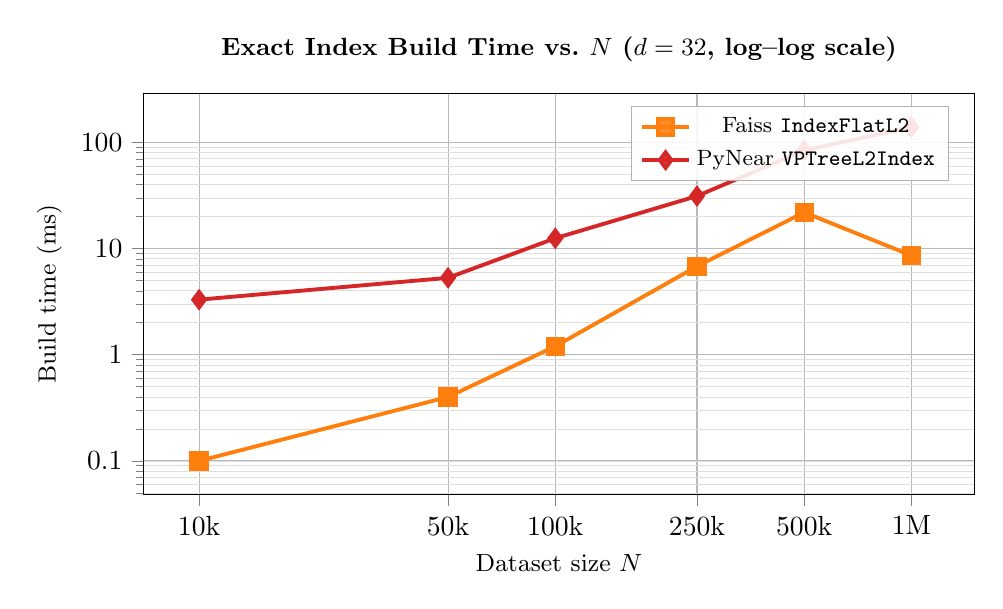
\begin{tikzpicture}
\begin{axis}[
  benchstyle,
  title={Exact Index Build Time vs.\ $N$
         ($d=32$, log--log scale)},
  xlabel={Dataset size $N$},
  ylabel={Build time (ms)},
  xmode=log, ymode=log,
  xtick={10000,50000,100000,250000,500000,1000000},
  xticklabels={10k,50k,100k,250k,500k,1M},
  xmin=7000, xmax=1500000,
  log ticks with fixed point,
  minor tick num=4,
]

% Faiss IndexFlatL2
\addplot[color=colOrange, mark=square*]
  coordinates {(10000,0.1)(50000,0.4)(100000,1.2)(250000,6.8)(500000,21.9)(1000000,8.6)};
\addlegendentry{Faiss \texttt{IndexFlatL2}}

% PyNear VPTreeL2Index
\addplot[color=colRed, mark=diamond*]
  coordinates {(10000,3.3)(50000,5.3)(100000,12.5)(250000,31.2)(500000,83.9)(1000000,139.2)};
\addlegendentry{PyNear \texttt{VPTreeL2Index}}

\end{axis}
\end{tikzpicture}
\caption{Exact-index build time (ms, log--log) vs.\ dataset size $N$, $d=32$.
  Faiss \texttt{IndexFlatL2} requires no structural work (copy only), giving
  an $O(N)$ lower bound (its non-monotonic 500k/1M points reflect allocator
  noise at sub-25-ms timescales).  \texttt{VPTreeL2Index} follows an
  $O(N \log N)$ curve, from 3.3 ms at $N=10\,000$ to 139 ms at $N=10^6$ —
  well within one-second build budgets for all tested sizes.}
\label{fig:build-exact}
\end{figure}

The $O(N \log N)$ growth of \texttt{VPTreeL2Index} results in a build-time
overhead of roughly $4\text{--}16\times$ vs.\ Faiss's copy-only flat index
at large $N$, which is expected and acceptable: the VP-Tree build cost is
paid once (139 ms for $10^6$ points) and amortised over all subsequent
queries, which benefit from tree pruning with leaf-bucketed SIMD sweeps
rather than an $O(N)$ linear scan — yielding $4\text{--}11\times$ lower
query latency at $d=32\text{--}128$ (Section~\ref{sec:l2-high}).
The build is level-parallel: all nodes at each tree depth are processed
concurrently with per-thread scratch buffers.  On Linux systems where Intel
TBB is available, \texttt{std::execution::par\_unseq} is additionally
applied to \texttt{nth\_element} at the root partition; on macOS and
TBB-free Linux environments the standard serial \texttt{nth\_element} is
used instead.

\subsection{Approximate Index: IVFFlatL2Index vs.\ Faiss IndexIVFFlat}
\label{sec:build-approx-scale}

Figure~\ref{fig:build-approx} plots build time for both IVF-style approximate
indices.  The number of clusters is $k = \lfloor\sqrt{N}\rfloor$ in all
cases, so the K-Means problem grows with $N$.

\begin{figure}[h]
\centering
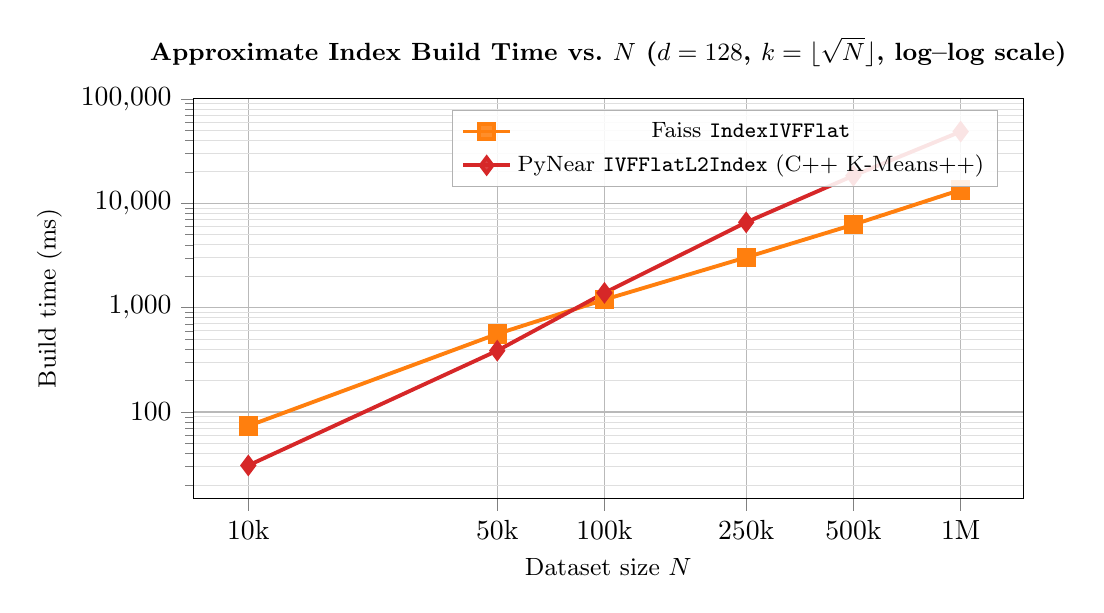
\begin{tikzpicture}
\begin{axis}[
  benchstyle,
  title={Approximate Index Build Time vs.\ $N$
         ($d=128$, $k=\lfloor\sqrt{N}\rfloor$, log--log scale)},
  xlabel={Dataset size $N$},
  ylabel={Build time (ms)},
  xmode=log, ymode=log,
  xtick={10000,50000,100000,250000,500000,1000000},
  xticklabels={10k,50k,100k,250k,500k,1M},
  xmin=7000, xmax=1500000,
  log ticks with fixed point,
  minor tick num=4,
]

% Faiss IndexIVFFlat
\addplot[color=colOrange, mark=square*]
  coordinates {(10000,73.6)(50000,560.1)(100000,1193.4)(250000,3031.1)(500000,6239.6)(1000000,13435.7)};
\addlegendentry{Faiss \texttt{IndexIVFFlat}}

% PyNear IVFFlatL2Index (C++ K-Means++)
\addplot[color=colRed, mark=diamond*]
  coordinates {(10000,30.8)(50000,387.2)(100000,1385.7)(250000,6565.8)(500000,18374.1)(1000000,48549.1)};
\addlegendentry{PyNear \texttt{IVFFlatL2Index} (C++ K-Means++)}

\end{axis}
\end{tikzpicture}
\caption{Approximate-index build time (ms, log--log) vs.\ dataset size $N$,
  $d=128$, $k = \lfloor\sqrt{N}\rfloor$.
  \texttt{IVFFlatL2Index} (C++ K-Means++ with SIMD + OpenMP) is
  \emph{faster} than Faiss \texttt{IndexIVFFlat} at $N \le 50\,000$
  (31 ms vs.\ 74 ms at $N=10\,000$; 387 ms vs.\ 560 ms at $N=50\,000$).
  At larger $N$ Faiss's highly optimised compiled K-Means takes over,
  reaching ${\sim}3.6\times$ faster at $N=10^6$.}
\label{fig:build-approx}
\end{figure}

\begin{table}[h]
\centering
\caption{Build time (ms) vs.\ $N$ for approximate IVF indices ($d=128$,
  $k=\lfloor\sqrt{N}\rfloor$).  \textbf{Bold} marks the faster method.}
\label{tab:build-scale}
\renewcommand{\arraystretch}{1.25}
\begin{tabular}{rcc}
\toprule
\textbf{N} & \textbf{IVFFlatL2 (C++ K-Means++)} & \textbf{Faiss IndexIVFFlat} \\
\midrule
10\,000  & \textbf{31}    & 74    \\
50\,000  & \textbf{387}   & 560   \\
100\,000 & 1\,386  & \textbf{1\,193}  \\
250\,000 & 6\,566  & \textbf{3\,031}  \\
500\,000 & 18\,374 & \textbf{6\,240}  \\
1\,000\,000 & 48\,549 & \textbf{13\,436} \\
\bottomrule
\end{tabular}
\end{table}

The crossover from PyNear-faster to Faiss-faster occurs between $N=50\,000$
and $N=100\,000$.  Below that threshold the C++ K-Means++ kernel
($\approx k=100\text{--}224$ clusters) enjoys a start-up advantage
($2.4\times$ faster at $N=10\,000$) — Faiss
allocates more resources for its K-Means iteration budget.  Above $N=100\,000$
Faiss's compiled BLAS-based centroid updates dominate, reaching
$3.6\times$ faster at $N=10^6$.
For large-scale workloads ($N \ge 250\,000$) users requiring short build
times may prefer Faiss IVF; for small-to-medium datasets \texttt{IVFFlatL2Index}
is the faster choice while offering the same Python-only install footprint.

% =============================================================================
\section{Discussion}
\label{sec:discussion}

\paragraph{Low-to-moderate dimensionality ($d \leq 64$).}
VP-Trees offer the best exact-search latency in this regime across all three
distance metrics tested ($\ell_1$, $\ell_2$, $\ell_\infty$).  The tree's
metric-space pruning criterion eliminates a substantial fraction of distance
evaluations, and with v2.4's 32-point leaf buckets the evaluations that do
occur run as contiguous SIMD sweeps, keeping latency essentially flat
(0.4--0.9 ms) even at $N = 2.5\times10^6$.
scikit-learn's kd-tree degrades rapidly beyond $d = 8$ due to increasing
overlap between ball partitions; Faiss's flat scan is memory-bandwidth-bound
and grows steadily with both $d$ and $N$.

\paragraph{Moderate-to-high dimensionality ($d = 32\text{--}128$) — exact.}
\texttt{VPTreeL2Index} remains the most efficient exact method at $d=128$
(0.49 ms vs.\ 5.3 ms for Faiss flat, 40.8 ms for scikit-learn), an
$11\times$ advantage over Faiss.  The tree's pruning effectiveness
degrades with dimension — a manifestation of the concentration of measure
phenomenon — and this edition's exact float suite deliberately stops at
$d=128$; beyond that the approximate indices below are the appropriate
tool.

\paragraph{High dimensionality ($d = 128\text{--}1024$) — approximate.}
\texttt{IVFFlatL2Index} maintains perfect Recall@10 at
$n_{\mathrm{probe}}=20$ with 0.18--0.67 ms per query, but the raw-latency
comparison has reversed since the previous edition: Faiss
\texttt{IndexIVFFlat} is now faster at every tested dimensionality
($8\text{--}32\times$ at $n_{\mathrm{probe}}=20$).  Where PyNear's IVF
retains an edge is build time — $1.4\text{--}2.4\times$ faster than Faiss
at $N = 50\,000$ across $d=128$--$1024$, and faster overall up to
$N \approx 10^5$ — plus the pure-Python install footprint and the
exact-search fallback via $n_{\mathrm{probe}} = n_{\mathrm{clusters}}$.
For raw approximate query throughput at high dimensionality, Faiss IVF is
the better choice on this hardware.

\paragraph{Binary descriptors — exact.}
Faiss's flat binary index is the fastest exact binary search method at
32--128 bits, but at 256 bits \texttt{VPTreeBinaryIndex} (v2.4,
leaf-bucketed popcount sweeps) is now $2.3\times$ faster (15.9 ms vs.\
36.3 ms in-process).  Since the exact suite times Faiss in the same
process as PyNear, its numbers may be depressed by the OpenMP runtime
clash (Section~\ref{sec:setup}); the subprocess-isolated measurement of
Section~\ref{sec:approx-binary} remains the fair reference for Faiss's
brute-force throughput.
\texttt{BKTreeBinaryIndex} is best suited to range queries
(\texttt{find\_threshold}), where its B-K tree structure is optimal, and
should not be interpreted as a general-purpose $k$-NN competitor.

\paragraph{Binary descriptors — approximate.}
\texttt{MIHBinaryIndex} and \texttt{IVFFlatBinaryIndex}
(Section~\ref{sec:approx-binary}) decisively outperform exact brute-force
binary search in the wide-descriptor, near-duplicate regime: at $d=512$,
$N=10^6$, MIH reaches 0.0088 ms/query (114\,039 QPS) at 100\% Recall@10,
$34\times$ faster than the thread-matched Faiss \texttt{IndexBinaryFlat}
scan, with Faiss's own MIH three orders of magnitude behind.  On narrow
128-bit descriptors the picture is more nuanced: \texttt{IVFFlatBinaryIndex}
offers the best throughput at the recall ceiling (56\,859 QPS at 0.845),
while an optimised brute-force scan beats MIH above the ${\sim}0.5$ recall
mark.  Choose MIH for wide descriptors and small-radius/near-duplicate
retrieval; choose IVF or brute force for high-recall search on narrow
descriptors.

% =============================================================================
\section{Conclusion}
\label{sec:conclusion}

PyNear's VP-Tree family provides highly competitive exact $k$-nearest-neighbour
search across $\ell_1$, $\ell_2$, and $\ell_\infty$ distance metrics,
delivering the lowest latency among all evaluated exact methods across the
full tested dimensionality range ($d = 2\text{--}128$) without requiring BLAS,
GPU, or any native runtime dependency beyond NumPy.
Version 2.4's leaf bucketing — 32-point leaves scanned as contiguous SIMD
sweeps, with best-first descent and pooled per-query heaps — keeps exact
query latency in the 0.4--0.9 ms band even at $N = 2.5\times10^6$
(low-dimensional suite) and at 0.49 ms for $d=128$, $N=120\,000$:
$11\times$ faster than Faiss \texttt{IndexFlatL2} and $83\times$ faster
than scikit-learn at that dimensionality.  It also carries the exact binary
index past Faiss at wide descriptors: at 256 bits,
\texttt{VPTreeBinaryIndex} is $2.3\times$ faster than
\texttt{IndexBinaryFlat} measured in-process.  The SIMD-accelerated
distance kernels keep all three float metric variants within a narrow
0.23--0.68 ms band, allowing practitioners to
select the semantically appropriate metric without performance penalties.

In the approximate $\ell_2$ regime, \texttt{IVFFlatL2Index} sustains
perfect Recall@10 at $n_{\mathrm{probe}}=20$ with sub-millisecond per-query
latency, and its C++ K-Means++ builder constructs the index
$1.4\text{--}2.4\times$ faster than Faiss IVF at $N=50\,000$ (crossover
near $N=10^5$; Faiss builds $3.6\times$ faster at $N=10^6$).  On raw query
latency, however, Faiss \texttt{IndexIVFFlat} now leads at every tested
dimensionality — PyNear's IVF value proposition is the build speed at small
$N$, the NumPy-only footprint, and the single-parameter exact fallback,
not peak throughput.

For approximate binary search, \texttt{MIHBinaryIndex} delivers a
$34\times$ speedup over a thread-matched exact brute-force scan on 512-bit
near-duplicate retrieval at $N=10^6$ with 100\% Recall@10, and
\texttt{IVFFlatBinaryIndex} reaches the SIFT1M recall ceiling at
$2.4\times$ the throughput of exact search — while on narrow descriptors
at high recall, exact brute force remains the honest recommendation.

Future work includes evaluating the exact float suite beyond $d=128$ under
the new leaf-bucketed traversal, narrowing the raw-latency gap of
\texttt{IVFFlatL2Index} through a compiled inner scan,
product-quantisation-based inner-cluster compression, and
evaluating performance on non-clustered (adversarial) data distributions.

\paragraph{Static index limitation.}
A notable architectural constraint of the current implementation is that all
PyNear indices are \emph{static}: the full tree must be reconstructed via
\texttt{set(data)} whenever the underlying dataset is modified.  No
incremental insertion, deletion, or in-place point update is supported.
This precludes direct use in workloads where the dataset evolves continuously,
most notably real-time physics simulation.  In particle-based simulation
systems (SPH fluids, cloth, soft-body dynamics), nearest-neighbour queries
must reflect the current particle positions after every integration step;
rebuilding a VP-Tree at each frame is prohibitively expensive.  Production
physics engines address this with structures designed for dynamic updates:
dynamic Bounding Volume Hierarchies (DBVH), incremental kd-trees, or spatial
hashing with temporal coherence.  Dynamic VP-Tree variants that support
$O(\log n)$ insertions and deletions have been studied in the
literature~\cite{yianilos1993data} and represent a natural direction for
future development of PyNear.

% =============================================================================
\begin{thebibliography}{9}

\bibitem{yianilos1993data}
P.~N. Yianilos,
\textit{Data structures and algorithms for nearest neighbor search in general
metric spaces},
in \textit{Proc.\ 4th ACM--SIAM Symposium on Discrete Algorithms (SODA)},
pp.~311--321, 1993.

\bibitem{johnson2019billion}
J.~Johnson, M.~Douze, and H.~J{\'{e}}gou,
\textit{Billion-scale similarity search with GPUs},
\textit{IEEE Transactions on Big Data}, vol.~7, no.~3, pp.~535--547, 2021.

\bibitem{pedregosa2011scikit}
F.~Pedregosa \textit{et al.},
\textit{Scikit-learn: Machine learning in Python},
\textit{Journal of Machine Learning Research}, vol.~12, pp.~2825--2830, 2011.

\bibitem{bernhardsson2018annoy}
E.~Bernhardsson,
\textit{Annoy: Approximate Nearest Neighbors Oh Yeah},
\url{https://github.com/spotify/annoy}, 2018.

\end{thebibliography}

\end{document}
